%% 
%% Copyright 2007-2020 Elsevier Ltd
%% 
%% This file is part of the 'Elsarticle Bundle'.
%% ---------------------------------------------
%% 
%% It may be distributed under the conditions of the LaTeX Project Public
%% License, either version 1.2 of this license or (at your option) any
%% later version.  The latest version of this license is in
%%    http://www.latex-project.org/lppl.txt
%% and version 1.2 or later is part of all distributions of LaTeX
%% version 1999/12/01 or later.
%% 
%% The list of all files belonging to the 'Elsarticle Bundle' is
%% given in the file `manifest.txt'.
%% 
%% Template article for Elsevier's document class `elsarticle'
%% with harvard style bibliographic references

%\documentclass[preprint,12pt,authoryear]{elsarticle}

%% Use the option review to obtain double line spacing
%% \documentclass[authoryear,preprint,review,12pt]{elsarticle}

%% Use the options 1p,twocolumn; 3p; 3p,twocolumn; 5p; or 5p,twocolumn
%% for a journal layout:
%% \documentclass[final,1p,times,authoryear]{elsarticle}
%% \documentclass[final,1p,times,twocolumn,authoryear]{elsarticle}
%% \documentclass[final,3p,times,authoryear]{elsarticle}
%% \documentclass[final,3p,times,twocolumn,authoryear]{elsarticle}
%% \documentclass[final,5p,times,authoryear]{elsarticle}
 \documentclass[final,5p,times,twocolumn, nopreprintline]{elsarticle}

%% For including figures, graphicx.sty has been loaded in
%% elsarticle.cls. If you prefer to use the old commands
%% please give \usepackage{epsfig}

%% The amssymb package provides various useful mathematical symbols
\usepackage{amssymb}
\usepackage{lipsum}
\usepackage{amsmath}
%\usepackage[pdftex,active,tightpage]{preview}
%\setlength\PreviewBorder{2mm}
\usepackage[spanish]{babel}
\usepackage{tikz}
\usepackage{pgfplots}
\pgfplotsset{compat=1.10}
\usepgfplotslibrary{fillbetween}
\usetikzlibrary{decorations.pathmorphing,patterns,calc,angles,positioning,babel,arrows.meta,plotmarks}
%% The amsthm package provides extended theorem environments
%% \usepackage{amsthm}

%% The lineno packages adds line numbers. Start line numbering with
%% \begin{linenumbers}, end it with \end{linenumbers}. Or switch it on
%% for the whole article with \linenumbers.
%% \usepackage{lineno}

%% You might want to define your own abbreviated commands for common used terms, e.g.:
\newcommand{\kms}{km\,s$^{-1}$}
\newcommand{\msun}{$M_\odot}
\newcommand{\toplrarr}[1]{\overset{\text{\scriptsize$\leftrightarrow$}}{#1}}
\numberwithin{equation}{section}
%\journal{Astronomy $\&$ Computing}

\begin{document}

\begin{frontmatter}

%% Title, authors and addresses

%% use the tnoteref command within \title for footnotes;
%% use the tnotetext command for theassociated footnote;
%% use the fnref command within \author or \affiliation for footnotes;
%% use the fntext command for theassociated footnote;
%% use the corref command within \author for corresponding author footnotes;
%% use the cortext command for theassociated footnote;
%% use the ead command for the email address,
%% and the form \ead[url] for the home page:
%% \title{Title\tnoteref{label1}}
%% \tnotetext[label1]{}
%% \author{Name\corref{cor1}\fnref{label2}}
%% \ead{email address}
%% \ead[url]{home page}
%% \fntext[label2]{}
%% \cortext[cor1]{}
%% \affiliation{organization={},
%%            addressline={}, 
%%            city={},
%%            postcode={}, 
%%            state={},
%%            country={}}
%% \fntext[label3]{}

\title{Parcial 3 Astrofísica Galáctica y Extragaláctica: parte práctica}

%% use optional labels to link authors explicitly to addresses:
%% \author[label1,label2]{}
%% \affiliation[label1]{organization={},
%%             addressline={},
%%             city={},
%%             postcode={},
%%             state={},
%%             country={}}
%%
%% \affiliation[label2]{organization={},
%%             addressline={},
%%             city={},
%%             postcode={},
%%             state={},
%%             country={}}

\author[first]{Santiago Julio Dávila 1000413445}
\affiliation[first]{organization={Instituto de Física, Universidad de Antioquia},%Department and Organization
            city={Medellín},
            state={Antioquia},
            country={Colombia}}


%\begin{abstract}
%%% Text of abstract
%
%\end{abstract}

%%Graphical abstract
%\begin{graphicalabstract}
%\includegraphics{grabs}
%\end{graphicalabstract}

%%Research highlights
%\begin{highlights}
%\item Research highlight 1
%\item Research highlight 2
%\end{highlights}

%\begin{keyword}
%%% keywords here, in the form: keyword \sep keyword, up to a maximum of 6 keywords
%antiparticle \sep Klein-Gordon equation \sep Klein paradox \sep pair production \sep particle \sep potential step \sep reflection and transmission coefficients \sep relativistic
%%% PACS codes here, in the form: \PACS code \sep code
%
%%% MSC codes here, in the form: \MSC code \sep code
%%% or \MSC[2008] code \sep code (2000 is the default)
%
%\end{keyword}


\end{frontmatter}

%\tableofcontents

%% \linenumbers

%% main text

\section{Distribución de partículas con simetría esférica}

El objetivo de esta sección del trabajo es estudiar extensivamente una distribución de 200000 partículas que constituyen un sistema no colisional con simetría esférica. Para esto, fueron provistos los datos de sus coordenadas $(x,y,z)$ en kpc y sus velocidades $(v_x,v_y,v_z)$ en km/s. Como se trata de un sistema con simetría esférica, se hizo necesario hacer la respectiva conversión de las posiciones y las velocidades a coordenadas esféricas, a través de las siguientes transformaciones:

\begin{align}
r=\sqrt{x^2+y^2+z^2} \label{eq:r}\\
\theta = \arccos\left(\frac{z}{\sqrt{x^2+y^2}}\right) \label{eq:th}\\
\phi = \mathrm{arg}\{x+iy\} \label{eq:ph}
\end{align}

para las coordenadas y

\begin{equation}
\begin{bmatrix}
v_r\\v_\theta\\v_\phi
\end{bmatrix} = \begin{bmatrix}
\sin\theta\cos\phi & \sin\theta\sin\phi & \cos\theta\\
\cos\theta\cos\phi & \cos\theta\sin\phi & -\sin\theta\\
-\sin\phi & \cos\phi & 0
\end{bmatrix}\begin{bmatrix}
v_x\\v_y\\v_z
\end{bmatrix} \label{eq:velesf}
\end{equation}

para las velocidades \cite{soto2009fisica}. Se define además un conjunto de unidades naturales para este sistema, a saber:

\begin{align}
U_M = 10^10~M_\odot \label{eq:UM}\\
U_L = 1~\text{kpc} \label{eq:UL}\\
U_T = 1.1~\text{Gyr} \label{eq:UT}\\
U_V = 1~\text{km/s} \label{eq:UV}\\
G = 43007.1 \label{eq:G}
\end{align}

\subsection{Isotropía}

Un primer indicio de que el sistema es isotrópico está en su tensor de dispersión de velocidades, que se define como 

\begin{equation}
\sigma^2_{ij}=\overline{v_iv_j}-\overline{v_i}\overline{v_j}. \label{eq:sigma2}
\end{equation}

El tensor de dispersión de velocidades se denomina \emph{isotrópico} si es diagonal en todo $\vec{r}$ y sus valores diagonales son iguales: $\sigma^2_{ij}=\sigma^2\delta_{ij}$ \cite{binney2011galactic}. Globalmente, se obtienen los siguientes tensores de dispersión de velocidades para los datos provistos a dos cifras decimales:

\begin{equation}
\boldsymbol{\sigma}^2_{cart}=\begin{bmatrix}
1121.20 & -2.34 & -2.37\\
-2.34 & 1111.76 & -0.25\\
-2.37 & -0.25 & 1122.47
\end{bmatrix}\label{eq:sigmacart}
\end{equation}

en coordenadas cartesianas y

\begin{equation}
\boldsymbol{\sigma}^2_{esf}=\begin{bmatrix}
1118.18 & 3.14 & -1.75\\
3.14 & 1119.87 & 2.38\\
-1.75 & 2.38 & 1117.36
\end{bmatrix}.\label{eq:sigmaesf}
\end{equation}

Nótese que en ambos tensores los valores diagonales son aproximadamente iguales, y los valores extradiagonales son al menos tres órdenes de magnitud menores que los valores diagonales, lo que es un buen indicador de que el sistema en cuestión es isotrópico. En definitiva, lo que determina si el sistema es, en efecto, isotrópico es el \emph{parámetro de anisotropía}, definido por

\begin{equation}
\beta(r)=1-\dfrac{\overline{v_\theta^2}+\overline{v_\phi^2}}{2\overline{v_r^2}}=1-\dfrac{\sigma_\theta^2+\sigma_\phi^2}{2\sigma_r^2}, \label{eq:beta}
\end{equation}

sistemas con $\beta<0$ se dice que son \emph{sesgados tangencialmente}, en tanto las dispersiones tangenciales dominan sobre la dispersión radial; sistemas con $\beta>0$ se llaman \emph{sesgados radialmente} y sistemas con $\beta=0$ son isotrópicos y ergódicos \cite{binney2011galactic}. Para todo el sistema, se obtiene un parámetro de anisotropía de

\begin{equation}
\beta_{tot}=-0.00039, \label{eq:betatot}
\end{equation}

y en general, se encuentra que $\beta(r)$ oscila en tre valores cercanos a 0, esto se hizo tomando cascarones esféricos delgados y calculando $\beta$ para las partículas en su interior. Para verificar que efectivamente se puede considerar que $\beta(r)\approx0$, se hizo un método de muestreo de \emph{bootstrapping} y se buscó que $\beta=0$ estuviese incluido en un intervalo de confianza del 95 \% para diferentes valores de $r$ \cite{vsirca2016probability,davison1997bootstrap}, obteniéndose los resultados mostrados en la figura \ref{fig:beta}.

\begin{figure}[h!]
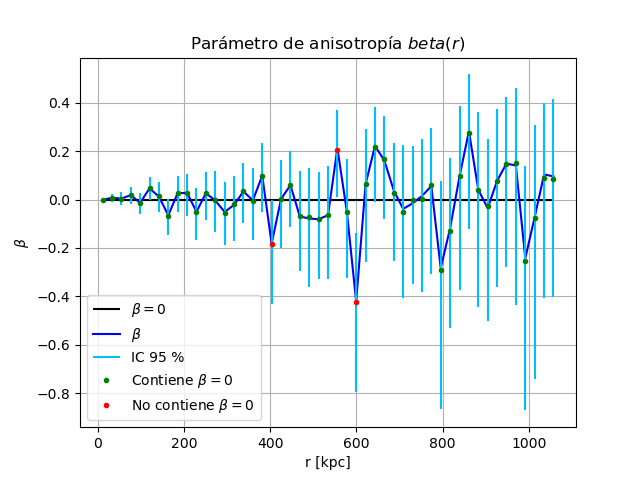
\includegraphics[width=\columnwidth]{../beta.png} 
\caption{$\beta(r)$ para el sistema de estudio. En la figura se observan los intervalos de confianza de 95 \% para cada uno de los $r$ y además se muestran los $r$ en cuyo intervalo de confianza se encuentra incluido $\beta=0$ y aquellos en los que no.}
\label{fig:beta}
\end{figure}

En la figura \ref{fig:beta} se observa que de los 50 cascarones considerados, solo hay dos en los que no se encuentra $\beta=0$ con un 95 \% de probabilidad. Esto es suficiente para asumir el valor de beta en la ecuación \ref{eq:betatot} como significativo y concluir que el sistema es isotrópico.

\subsection{Equilibrio estacionario}

Un sistema en equilibrio estacionario se define como aquel cuya densidad no depende explícitamente del tiempo:

\begin{equation}
\dfrac{\partial\rho}{\partial t}=0. \label{eq:stat}
\end{equation}

En términos de observables, un indicativo de que el sistema está en equilibrio estacionario es que sus velocidades medias sean nulas, sin embargo, esto no es una condición suficiente para probarlo. De los datos, se obtiene que las velocidades cartesianas medias en km/s son

\begin{align*}
\overline{v_x}=2.425\times10^{-9}\\
\overline{v_y}=2.28\times10^{-9}\\
\overline{v_z}=-4.535\times10^{-9}.
\end{align*}

Procediendo de manera análoga a como se hizo para el parámetro de anisotropía, se hizo un muestreo de bootstrapping para determinar la validez de estas medias, obteniendo los resultados mostrados en la figura \ref{fig:vs}.

\begin{figure}[h!]
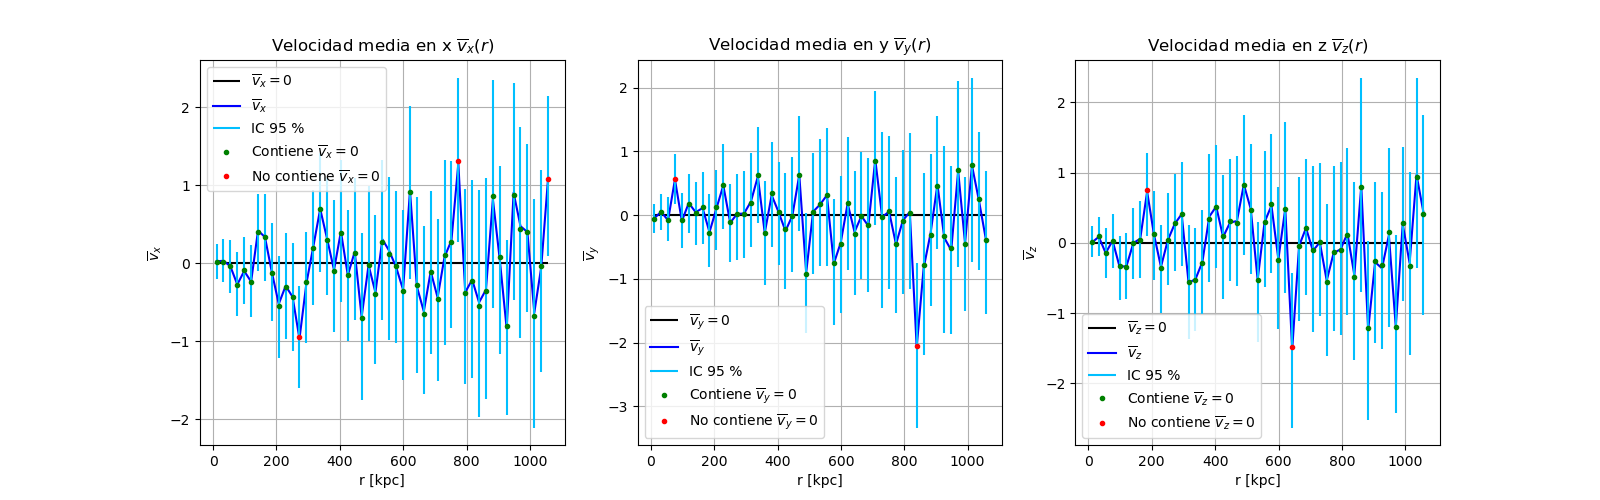
\includegraphics[width=\columnwidth]{../vm.png} 
\caption{$\overline{v_i}(r)$ para el sistema de estudio. En la figura se observan los intervalos de confianza de 95 \% para cada uno de los $r$ y además se muestran los $r$ en cuyo intervalo de confianza se encuentra incluido $\overline{v_i}=0$ y aquellos en los que no.}
\label{fig:vs}
\end{figure}

Nuevamente, se observa que solo hay, como máximo, tres valores de $r$ en los cuales $v_i=0$ no se encuentra con un 95 \% de probabilidad, lo que indica que los valores de las velocidades medias son verdaderos y el sistema podría estar en equilibrio estacionario.

No obstante, sí se puede obtener una condición suficiente para verificar si el sistema está en equilibrio estacionario, y se define a través de la ecuación de continuidad \cite{pathria}

\begin{equation}
\dfrac{\partial\rho}{\partial t}+\nabla\cdot(\rho\langle\vec{v}\rangle)=0. \label{eq:cont}
\end{equation}

Nótese que si la divergencia en la ecuación \ref{eq:cont} se anula, inmediatamente se concluye que la densidad no depende explícitamente del tiempo. La divergencia nula indica que no hay flujo de partículas en un volumen de control definido y, por tanto, no hay un cambio temporal en la densidad. Como el sistema tiene simetría esférica, se escoge este sistema de coordenadas para calcular la divergencia, y además no hay dependencia de los ángulos en las cantidades físicas involucradas, de modo que 

\begin{equation}
\nabla\cdot(\rho\langle\vec{v}\rangle)=\dfrac{1}{r^2}\dfrac{\partial}{\partial r}(r^2\rho v_r). \label{eq:div}
\end{equation}

Al calcular esta divergencia para el sistema de estudio se obtiene la gráfica \ref{fig:div}.

\begin{figure}[!ht]
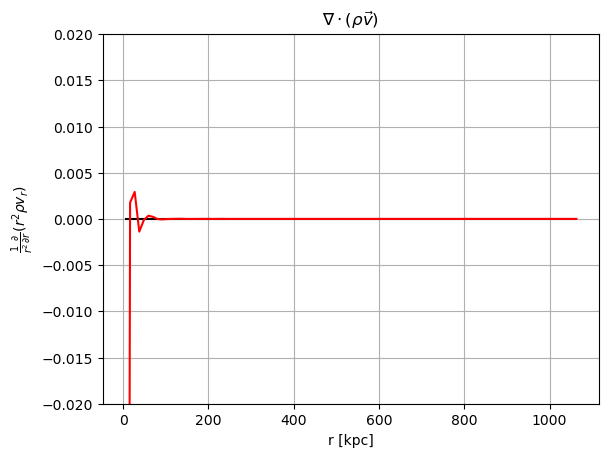
\includegraphics[width=\columnwidth]{../div.png}
\caption{Término de flujo de partículas para el sistema de estudio.}
 \label{fig:div}
\end{figure}

Obsérvese que la divergencia tiene algunas fluctuaciones para valores bajos de $r$, esto se debe al factor $r^{-2}$ mostrado en la ecuación \ref{eq:div}, que hace que la divergencia sea singular en $r=0$, sin embargo, se ve que rápidamente se estabiliza en cero, de modo que se puede concluir que este término se anula en la ecuación de continuidad, dando lugar a la ecuación \ref{eq:stat} que define el equilibrio estacionario.

\subsection{Dispersión de velocidades}

Teniendo en cuenta que el sistema es isotrópico, se puede calcular la dispersión de velocidades calculando únicamente la dispersión en alguna de las componentes de la velocidad, por ejemplo, la radial. Este proceso se hizo tomando un total de 100 cascarones esféricos delgados y calculando la dispersión en las velocidades radiales de las partículas contenidas en cada cascarón, dando lugar a la gráfica \ref{fig:sigma}.

\begin{figure}[h!]
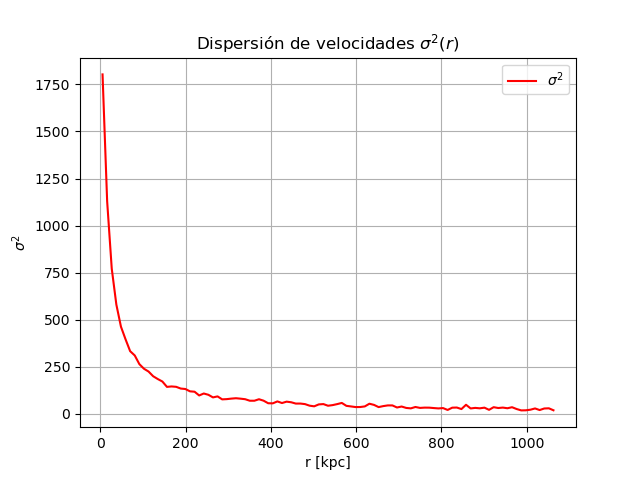
\includegraphics[width=\columnwidth]{../sig.png}
\caption{Dispersión de velocidades como función del radio.}
 \label{fig:sigma}
\end{figure}

Se puede observar el esperado comportamiento decreciente: en regiones más cercanas al centro del sistema habrá más energía disponible para imprimir en las partículas de modo que hay más dispersión en las velocidades que poseen las partículas, y esta dispersión se da de la misma manera en todas las direcciones debido a la isotropía del sistema; para valores grandes de $r$ se espera que la dispersión sea menor en tanto el sistema dispone de menos energía para darle a las partículas, de modo que las velocidades son más uniformes en las afueras del sistema.

\subsection{Masa total}

Considerando un sistema con simetría esférica, isotrópico y en equilibrio estacionario, la masa total del mismo se puede encontrar a través de las ecuaciones de Jeans \cite{binney2011galactic}, considerando

\begin{equation}
\dfrac{\mathrm{d}\Phi}{\mathrm{d}r}=\dfrac{GM(r)}{r^2}, \label{eq:gauss}
\end{equation}

donde $M(r)$ es la masa contenida dentro de una esfera de radio $r$. Así pues la masa acumulada del sistema es dada por

\begin{equation}
M(r)=-\dfrac{r\sigma^2}{G}\left(\dfrac{\mathrm{d}\ln n}{\mathrm{d}\ln r}+\dfrac{\mathrm{d}\ln \sigma^2}{\mathrm{d}\ln r}\right), \label{eq:mass}
\end{equation}

donde se usó el hecho de que el sistema está compuesto por $N$ partículas idénticas de masa $m$ constante, de modo que la densidad se puede escribir en términos de la densidad de número $n$ como $\rho=mn$\footnote{En lo sucesivo, se hará referencia a la densidad y a la densidad de número de manera indistinta.}. Nuevamente, la densidad de número se encontró usando cascarones: $n=dN_i/dV_i$, donde $dN_i$ es el número de partículas dentro del i-ésimo cascarón y $dV_i$ es el volumen del mismo, dando lugar a la distribución mostrada en la figura \ref{fig:dens}. Las derivadas logarítmicas en la ecuación \ref{eq:mass} se obtienen ajustando el logaritmo de los datos mostrados en las figuras \ref{fig:sigma} y \ref{fig:dens} a líneas rectas; recordando que lo que se quiere es estimar la masa total, el comportamiento de $\ln\rho(\ln r)$ y $\ln\sigma^2(\ln r)$ es aproximadamente lineal para valores de $r $ grandes como se muestra en la figura \ref{fig:fits}, de modo que la ecuación \ref{eq:mass}, evaluada en $r_{max}$, el radio máximo del sistema, da una aproximación a la masa total y queda escrita como:

\begin{equation}
M\simeq-\dfrac{r_{max}\sigma^2(r_{max})}{G}\left(m_\rho+m_{\sigma^2}\right), \label{eq:mass}
\end{equation}

donde $m_\rho,m_{\sigma^2}$ son las pendientes de los ajustes lineales a los logaritmos de la densidad y la dispersión de velocidades, respectivamente. Para los datos, el valor máximo de $r$ es de $r_{max}=1062.62$ kpc, y los valores de las pendientes encontrados fueron de $m_\rho=-3.775$ y $m_{\sigma^2}=-0.918$, dando lugar a una masa de $M=209.024~U_M=2.09\times10^12~M_\odot$, que es la masa típica del halo de materia oscura de una galaxia como la vía láctea, por ejemplo.

\begin{figure}[h!]
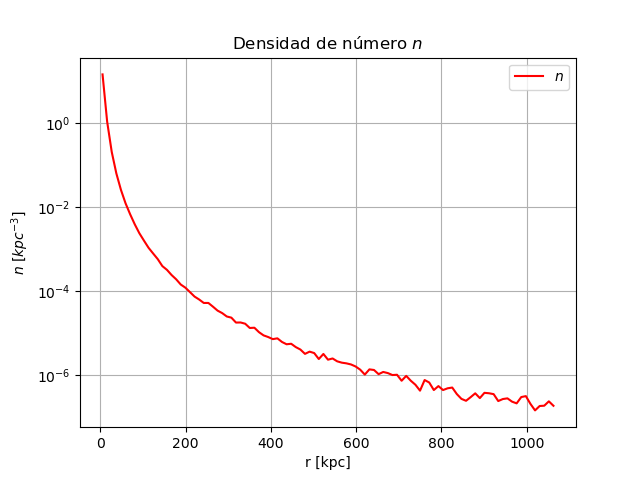
\includegraphics[width=\columnwidth]{../numdens.png}
\caption{Densidad de número como función del radio.}
 \label{fig:dens}
\end{figure}

\begin{figure}[h!]
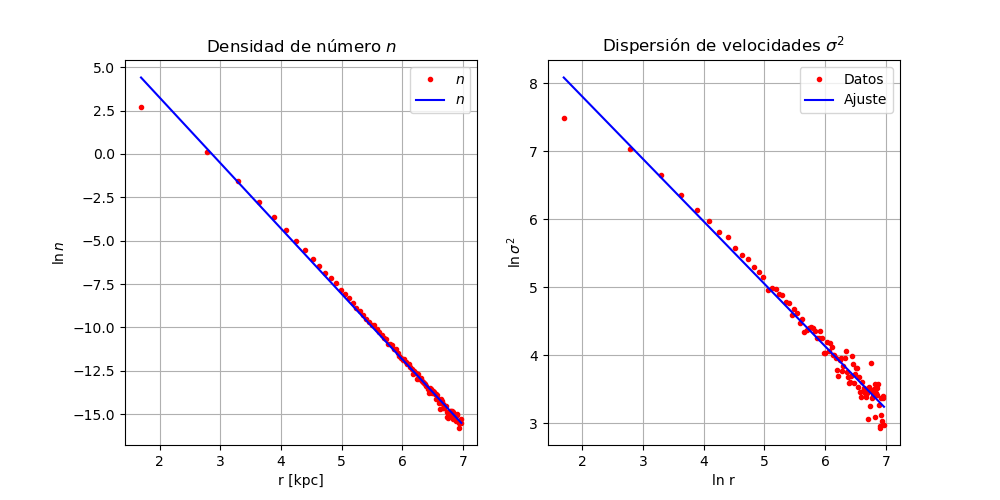
\includegraphics[width=\columnwidth]{../fit.png}
\caption{Ajustes lineales al logaritmo de la densidad y el logaritmo de la dispersión de velocidades.}
 \label{fig:fits}
\end{figure}

\bibliographystyle{unsrt} 
\bibliography{example.bib}





%% else use the following coding to input the bibitems directly in the
%% TeX file.

%%\begin{thebibliography}{00}

%% \bibitem[Author(year)]{label}
%% For example:

%% \bibitem[Aladro et al.(2015)]{Aladro15} Aladro, R., Martín, S., Riquelme, D., et al. 2015, \aas, 579, A101


%%\end{thebibliography}

\end{document}

\endinput
%%
%% End of file `elsarticle-template-harv.tex'.
